\documentclass[10pt]{ctexart}
\usepackage[paperwidth=36in,paperheight=24in,margin=0.4in]{geometry}
\usepackage{amsmath,amssymb,booktabs,graphicx,xcolor,hyperref}
\hypersetup{colorlinks=true,urlcolor=blue!50!black}
\pagestyle{empty}
\setlength{\parindent}{0pt}
\setlength{\parskip}{0.35em}
\graphicspath{{../../artifacts/extension/figures/}}
\InputIfFileExists{../../artifacts/extension/extension_macros.tex}{}{}
\definecolor{band}{HTML}{1B3A4B}
\definecolor{accent}{HTML}{C4492C}
\begin{document}
\fontsize{17}{21}\selectfont

\noindent\textcolor{band}{\fontsize{42}{46}\selectfont\bfseries Countdown 上的推理后训练}\\[0.05em]
{\fontsize{20}{24}\selectfont 长 think SFT 提供覆盖，在线 RL 把分布变尖，验证器收回已经采样到的解}\\[0.08em]
{\normalsize ShaneLiu04 \quad CS224R Default Project \quad Qwen2.5-0.5B \quad
\url{https://github.com/ShaneLiu04}}\\[0.06em]
{\color{band}\rule{\textwidth}{2.5pt}}\vspace{0.15em}

\noindent
\begin{minipage}[t]{0.315\textwidth}
{\color{accent}\bfseries\fontsize{22}{26}\selectfont 问题}\par\vspace{0.2em}
Countdown 给出几个整数和一个目标。模型必须每个数字恰好用一次，写出等于目标的等式。
没有 \texttt{<answer>} 时奖励是 $0$，格式对但算错是 $0.1$，等式正确是 $1$。
基座 Qwen2.5-0.5B 在留出集 $500$ 题上的 pass@1 是 $\xBaseHeldoutPassato$，
pass@16 是 $\xBaseHeldoutPassatos$。奖励几乎全是 $0$，组内优势也是 $0$，
策略梯度没有方向。

这件事值得单独做，是因为推理 RL 的论文常常只报 pass@1。
pass@1 上升可以是``更常一次命中''，也可以是``八次里至少一次''变多。
这两句话对产品的含义相反：前者是把质量收进单次采样，后者才是能力变宽。

\vspace{0.35em}{\color{accent}\bfseries\fontsize{22}{26}\selectfont 方法}\par\vspace{0.2em}
冷启动用长 \texttt{<think>} 的监督微调。在线阶段每步 $32$ 个提示、组大小 $8$、$100$ 步，
学习率 $10^{-5}$，熵和 KL 系数都是 $0.001$。vLLM 以温度 $1$ 采样，
每步把当前权重复制回去。三种优势共用序列对数概率之和：
\begin{align*}
A^{\mathrm{RLOO}}_i &= r_i - \tfrac{1}{K-1}\sum_{j\neq i} r_j,\\
A^{\mathrm{GRPO}}_i &= (r_i-\bar r)/(\sigma+\epsilon),\\
A^{\mathrm{Dr}}_i &= r_i-\bar r.
\end{align*}
Dr.\ GRPO 去掉的是标准差。损失没有再除以回答长度。
课程学习前一半只出三数字题，后一半只出四数字题。
短等式 SFT 是对照：格式对了，但没有长搜索。

测试时在 $k$ 条样本里重排。全验证器就是训练用的等式检查，题目里已经有目标和数字。
对照是均匀抽一条、多数投票、最大平均对数概率，以及只检查数字是否用全。
评估温度 $0.6$、top-$p$ $0.95$，每题 $16$ 条。留出 $500$ 题不进入训练。
\end{minipage}\hfill
\begin{minipage}[t]{0.35\textwidth}
{\color{accent}\bfseries\fontsize{22}{26}\selectfont 结果}\par\vspace{0.15em}
\begin{center}
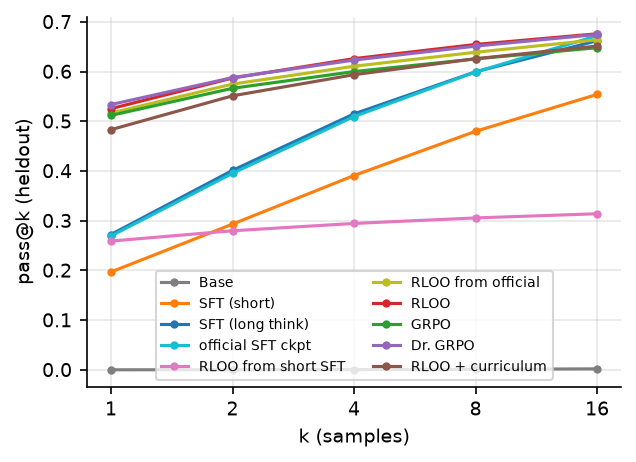
\includegraphics[width=0.92\linewidth]{ext_fig1_passk_heldout.png}
\end{center}
\vspace{-0.35em}
{\small 留出集 $500$ 题。在线方法的曲线更陡，右端几乎重合。$\pm$ 是种子间标准差。}

{\small
\begin{center}
\setlength{\tabcolsep}{4pt}
\begin{tabular}{@{}lcc@{}}
\toprule
 & pass@1 & pass@16 \\
\midrule
长 think SFT & $\xSftLongHeldoutPassato$ & $\xSftLongHeldoutPassatos$ \\
短等式 SFT & $\xSftShortHeldoutPassato$ & $\xSftShortHeldoutPassatos$ \\
RLOO & $\xRlRlooLongHeldoutPassato$ & $\xRlRlooLongHeldoutPassatos$ \\
GRPO & $\xRlGrpoLongHeldoutPassato$ & $\xRlGrpoLongHeldoutPassatos$ \\
Dr.\ GRPO & $\xRlDrgrpoLongHeldoutPassato$ & $\xRlDrgrpoLongHeldoutPassatos$ \\
课程学习 & $\xRlCurrLongHeldoutPassato$ & $\xRlCurrLongHeldoutPassatos$ \\
官方 SFT + RLOO & $\xRlRlooOfficialHeldoutPassato$ & $\xRlRlooOfficialHeldoutPassatos$ \\
短等式 + RLOO & $\xRlRlooShortHeldoutPassato$ & $\xRlRlooShortHeldoutPassatos$ \\
\bottomrule
\end{tabular}
\end{center}
}

pass@1 从 $0.27$ 附近升到 $0.52$--$0.54$，pass@16 仍在 $0.64$--$0.68$。
在线 RL 把概率质量推向已经会的题，没有把 $16$ 次采样的覆盖再拉开。
短等式初始化上的 RLOO 把 pass@16 打到 $\xRlRlooShortHeldoutPassatos$，低于它的 SFT。
同样的优势，坏的冷启动会把覆盖训掉。课程学习没有超过同一预算的普通 RLOO。
GRPO 和 Dr.\ GRPO 的差距还没有大过种子之间的起伏，不能把``去掉标准差''写成稳定排序。

\begin{center}
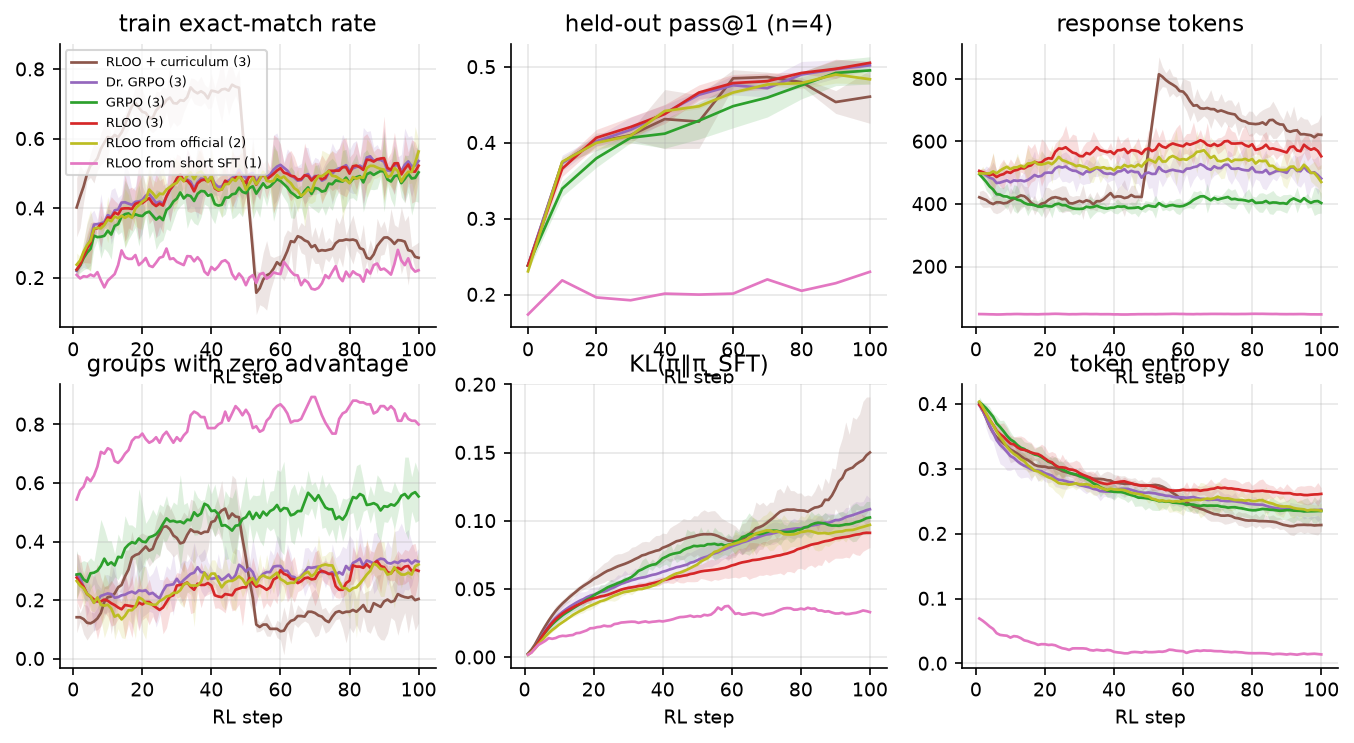
\includegraphics[width=\linewidth]{ext_fig7_rl_curves.png}
\end{center}
\vspace{-0.4em}
{\small 在线精确率。曲线在上升，但终点的 pass@16 没有离开 SFT。}
\end{minipage}\hfill
\begin{minipage}[t]{0.315\textwidth}
{\color{accent}\bfseries\fontsize{22}{26}\selectfont 重排与边界}\par\vspace{0.15em}
\begin{center}
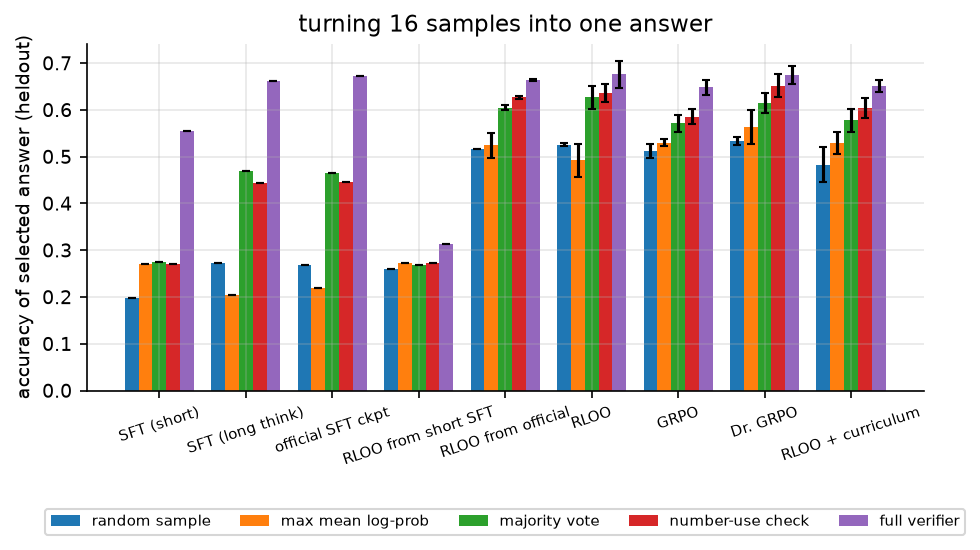
\includegraphics[width=\linewidth]{ext_fig2_selection_heldout.png}
\end{center}
\vspace{-0.6em}
{\small $k=16$ 的选择器。全验证器等于 pass@16。最大对数概率低于随机一条。}

全验证器能把小预算上的命中率拉向 pass@$k$，因为它丢掉算错的等式。
最大平均对数概率偏向短而流利的错答案，留出集上低于均匀抽取。
重排收回的是采样里已经出现的解。训练没覆盖到的题，检查器也挑不出来。

\vspace{0.3em}{\color{accent}\bfseries\fontsize{22}{26}\selectfont 可以带走的四句话}\par\vspace{0.15em}
\begin{enumerate}
\setlength{\itemsep}{0.45em}
\item 先看奖励是否有方差。基座 pass@1 是 $0$ 时，RLOO 的优势也是 $0$。
\item 同时报 pass@1 和 pass@16。只报前者会把``分布变尖''说成``学会了解题''。
\item 冷启动的格式要和奖励对齐。长 think 上 RL 抬高 pass@1；短等式上 RL 压低 pass@16。
\item 有便宜检查器时，测试时多采样再验证，比再训一个打分模型直接。对数概率不是这个检查器的替代品。
\end{enumerate}

\textbf{边界。}模型是 $0.5$B，不是论文里的大模型。在线预算是 $100$ 步、每步 $32$ 个提示，
不是官方 batch $128$ 再累积 $128$。种子间的标准差以
\texttt{extension\_macros.tex} 为准。评估温度和训练温度不同。
Dr.\ GRPO 在这里只比较了标准差缩放，没有比较长度归一化。

\vspace{0.4em}
{\color{band}\rule{\linewidth}{2pt}}\\
{\small 数字由 \texttt{analysis/plot\_extension.py} 从留出集 JSON 生成。
海报对应课程要求的四个问题：任务是什么、为什么值得做、实验看到了什么、听众能带走什么以及哪里不能外推。}
\end{minipage}
\end{document}
